\documentclass[12pt,oneside]{article}
\usepackage[paperheight=26cm,paperwidth=18.4cm]{geometry}
%\usepackage[paperwidth=9.2cm, paperheight=12.4cm, width=9cm, height=12cm,top=0.2cm,bottom=0.4cm,left=0.2cm,right=0.2cm,foot=0cm, nohead,nofoot]{geometry}
%\geometry{left=1cm,right=1cm,top=2cm,bottom=2cm}
\usepackage{anysize}
\papersize{26cm}{18.4cm}
\marginsize{1.5cm}{2.1cm}{2cm}{2cm} 
%\marginsize{1cm}{1cm}{1cm}{1cm} 

%\usepackage[utf8]{inputenc}
%\usepackage[T1]{fontenc}
\usepackage{fixltx2e}
\usepackage{graphicx}
\usepackage{longtable}
\usepackage{float}
\usepackage{wrapfig}
\usepackage{soul}
\usepackage{textcomp}
\usepackage{marvosym}
%\usepackage{wasysym}
\usepackage{latexsym}
\usepackage{amssymb}
%\usepackage{hyperref}
\tolerance=1000
\usepackage{etex}
\usepackage{amsmath}
\usepackage[usenames]{color}
\usepackage{pstricks}
\usepackage{pgfplots}
\usepackage{tikz}
\usepackage[europeanresistors,americaninductors]{circuitikz}
\usepackage{colortbl}
\usepackage{yfonts}
\usetikzlibrary{shapes,arrows,matrix}
\usetikzlibrary{positioning}
\usetikzlibrary{intersections}
\usetikzlibrary{calc,patterns,decorations.pathmorphing,decorations.markings}
\usepackage[BoldFont,SlantFont,CJKchecksingle,CJKnumber]{xeCJK}
\setCJKmonofont{Evermore Kai}
\setCJKmainfont[BoldFont=Evermore Hei]{Evermore Song}
\setCJKfamilyfont{hei}{Evermore Hei}
%\usepackage{CJKnumb}
%\xeCJKsetup{CJKglue=\hspace{0pt plus .08 \baselineskip }}
\usepackage{pst-node}
\usepackage{pst-plot}
\psset{unit=5mm}
%\pdfcompresslevel=9
\DeclareGraphicsExtensions{.jpg,.pdf,.mps,.png}

%\usepackage{CJK,CJKnumb}
\usepackage{listings}
\usepackage{tabularx}
\usepackage{longtable}
\usepackage{indentfirst}                % 首行缩进宏包
\usepackage{color}                      % 支持彩色
\usepackage{listings}                   % 源代码宏包
\usepackage[perpage,symbol]{footmisc}   % 脚注控制
\usepackage{lastpage}                   % 自动记录总页数宏包,计数器为LastPage
\usepackage{fancyhdr}                   % fancyhdr宏包 页眉和页脚的相关定义
\pagestyle{empty}
\topmargin -5mm \oddsidemargin -10mm \evensidemargin -10mm \textwidth 150mm \textheight 200mm
\headsep 1em
\pagestyle{fancyplain}                  % 要在\usepackage{pageno}之前,不然页眉有一条黑线去不掉
%\usepackage{pageno}                     % 章首页的页眉处理, 可以改为自己想要的形式 


\renewcommand{\baselinestretch}{1.5}
\allowdisplaybreaks


%----------------------------------页眉页脚---------------------------------------
%\pagestyle{fancyplain}
\renewcommand{\headrulewidth}{0pt}
\fancyhf[C]{西北工业大学命题专用纸}
\fancyfoot[C]%[RE][LO]
{ \hfill \\
教务处印制\hfill共\pageref{LastPage}页\quad第\thepage页}

\lfoot{\setlength{\unitlength}{1mm}
\begin{picture}(0,0)\linethickness{0.4mm}
\put(77,109){\makebox(0,0){\framebox(160,210){}}}
\end{picture}}
%---------------------------------------------------------------------------------


\begin{document}



%---------------------------------------源代码------------------------------------------------
\lstset{xleftmargin=1em,xrightmargin=1em}
\lstset{commentstyle=\textit,keywordstyle=\textbf,breaklines=true,columns=flexible,mathescape=true}
\lstdefinestyle{numbers}{numbers=left,stepnumber=1,numberstyle=\small,numbersep=1em}
\lstset{language=C++}
  \lstset{%
numbers=left,stepnumber=1,numberstyle=\tiny,
  %basicstyle=\footnotesize\ttfamily,
  basicstyle=\ttfamily,
  commentstyle=\textit,
  keywordstyle=\textbf,
  identifierstyle=\slshape,
  stringstyle=\small,
  %stringstyle=\color{orange},
  breaklines=true,
%    escapechar=\#,
    emphstyle=\bfseries\color{red}
}
\renewcommand{\lstlistingname}{程序}

%\CJKcaption{GB}
%\CJKcaption{gb_452}
%\CJKtilde \CJKindent

\newcounter{question}
\usecounter{question}
\setcounter{question}{1}
\newcommand{\question}{{\flushleft\CJKnumber{\arabic{question}}、}\stepcounter{question}}



%--------------------------------------首页页眉页脚---------------------------------------------
\fancypagestyle{plain}{%
\fancyhf{} % clear all header and footer fields
\renewcommand{\headrulewidth}{0pt}
\renewcommand{\footrulewidth}{0pt}
\fancyfoot[C]%[RE][LO]
{
\renewcommand{\baselinestretch}{1.0}
\begin{tabular}{ll} 
 注: &  命题纸上一般不留答题位置,试题请用小四、宋体打印且不出框。\\
% & 2. 命题教师和审题教师姓名应在试卷存档时填写。\hspace{3em} 共\pageref{LastPage}页 第\thepage页 
 &  \hspace{25em} 共\pageref{LastPage}页 第\thepage页 
\end{tabular}
}
\lfoot{\setlength{\unitlength}{1mm}
\begin{picture}(0,0)\linethickness{0.4mm}
\put(77,52){\makebox(0,0){\framebox(160,88.5){}}}
\put(-3,85.5){\line(1,0){160}}
\put(0,89){\raisebox{0ex}[4ex][2ex]{考生班级}\  \vline \hspace{8em}\hfill \vline\ 学\hspace{1em}号\ \vline \hspace{10em}\hfill \vline\ 姓\hspace{1em}名\ \vline\hfill  \hspace{6eM} }
\end{picture}}}
\thispagestyle{plain}
%------------------------------------------------------------------------------------------------
\setlength{\unitlength}{1ex}
\begin{center}

\begin{minipage}{84ex}
\parbox{84ex}{\CJKfamily{hei}
\center{诚信保证} \\ \vspace{-2ex}
\flushleft
\hspace{2eM}本人知晓我校考场规则和违纪处分条例的有关规定,保证遵守考场规则,诚实做人。\hfill 本人签字:\underline{\hspace{4eM}}\\ \vspace{1ex}}
\end{minipage}

\begin{picture}(0,0)

\put(0,7){\makebox(0,0){\dashbox(92,14){}
}}
\end{picture}

\end{center}

%\large
\noindent 编号:\underline {\hspace{4eM}}


%\vspace{-6ex}

\begin{center}
\textbf{ \fontsize{18pt}{\baselineskip}\selectfont{西北工业大学考试试题(卷)}}\\
2015 -2016 学年第 1 学期
\end{center}

{
\flushleft

\begin{tabular}{lll}
开课学院 \underline {\hspace{1em} 航天学院\hspace{1em} }& 课程\underline {\hspace{1em} 自动控制理论1\hspace{1em} }& 学时\underline {\hspace{1em} 48\hspace{1em} }\\
考试日期\underline {\hspace{6eM} }& 考试时间\underline {\hspace{1em} 2\hspace{1em} }小时 & 考试形式
$\left(\begin{array}{c}
\mbox{开}\\
\mbox{闭}
\end{array} \right)$
$\left(\begin{array}{*{10}c}
 \mbox{A} \\
 \mbox{B} 
\end{array} \right)$卷 
\end{tabular}
}

{
\center
%\renewcommand{\tabcolsep}{6pt}
\renewcommand{\tabcolsep}{1.2em}
\begin{tabular}{|c|c|c|c|c|c|c|c|c|c|} 
\hline
题号 & 一 & 二 & 三 & 四 & 五 & 六 & 七 & 八 & 总分 \\
\hline
得分 &    &    &    &    &    &    &    &    & \\
\hline 
\end{tabular}
}
\begin{tabular}{c}
\ \\
\ 
\end{tabular}
%\begin{minipage}{170mm}
%\ \raisebox{0ex}[4ex][2ex]{考生班级}\  \vline   \hfill \vline\ 学\hspace{1em}号\ \vline\hfill  \vline\ 姓\hspace{1em}名\ \vline\hfill  \hspace{6eM} \\
%\vskip -2.3ex \hrule
%\end{minipage}
\newcommand{\onlytest}[1]{#1}
\newcommand{\onlyanswer}[1]{}
%-----------------内容放在这里--------------------------

\question(20分) {已知系统结构图如图所示。求解前向通道传递函数{\Large $\frac{C(s)}{E(s)}$}与系统闭环传递函数{\Large $\frac{C(s)}{R(s)}$}。
	
	\includegraphics{image/diagram-2.pdf}
	
	\onlyanswer{
		解:
		
		\begin{eqnarray*}
			\frac{C(s)}{E(s)}&=&\frac{2G_1(s)G_2(s)+G_1(s)+G_2(s)}{1-G_1(s)G_2(s)}\\
			\frac{C(s)}{R(s)}&=&\frac{G(s)}{1-G(s)H(s)}\\
			&=&\frac{2G_1(s)G_2(s)+G_1(s)+G_2(s)}{1-G_1(s)G_2(s)-H(s)[2G_1(s)G_2(s)+G_1(s)+G_2(s)]}
		\end{eqnarray*}
	}
}


\onlytest{\vskip 3em}

\onlytest{\newpage}

\question(20分){已知某系统的结构图如图所示,分析是否可选取$k\in\mathbb{R}$的值,使系统在$r(t)=t^2$作用时,稳态误差$e_{ss}<0.5$ 。若是,则给出$k$的取值范围。

\includegraphics[scale=1.3]{image/diagram-1.pdf}

\onlyanswer
{
解:\\
\begin{eqnarray}
G(s) &=& \frac{k}{s}\cdot\frac{s+1}{s(s+3)(s+6)}\\
\Phi(s)&=&\frac{G(s)}{1+G(s)}\\
\frac{E(s)}{R(s)}&=&\frac{1}{1+G(s)}
\end{eqnarray}
首先考虑系统稳定性:
$$D(s)=S^2(s+3)(s+6)+k(s+1)=s^4+9s^3+18s^2+ks+k$$

Routh表:

\begin{tabular}{cccc}
	$s^4$: & 1 & 18 & k \\
	$s^3$: & 9 & k &\\
	$s^2$: & $18-\frac{k}{9}$ & k &\\
	$s^1$: & $k-\frac{9k}{18-\frac{k}{9}}$ & &\\
	$s^0$: & k & &
\end{tabular}

得:$$0<k<81$$

然后考虑动态指标$e_{ss}<0.5$:

因为:
$$R(s)=2\cdot\frac{1}{s^3}$$
所以:
$$e_{ss}=\lim_{s\rightarrow 0}{E(s)}=\frac{36}{k}$$
由$e_{ss}<0.5$得:
$$k>72$$
因此,$k$的范围是:
$$72<k<81$$
}
}


\question(20分) {单位负反馈系统开环传递函数
$$G(s)=\frac{K^*(s+3)}{s(s+2)}$$
求使系统闭环极点的实部均小于$-2$的$K^*$范围;证明系统非实轴上的根轨迹为圆,并求出其圆心与半径。

\onlyanswer{
解:

系统闭环传递函数为:
\begin{align*}
\Phi(s) &=\frac{K^*(s+3)}{K^*(s+3)+s(s+2)}\\
        &=\frac{K^*(s+3)}{K^*(s+3)+s(s+2)}\\
\end{align*}
设$s'=s+2$,将$s=s'-2$代入特征方程,
\begin{align*}
D(s') &=K^*(s'-2+3)+(s'-2)(s'-2+2)\\
      &=s'^2+(K^*-2)s'+K^*2
\end{align*}

利用Routh判据可知$K^*>2$ 时,闭环极点实部小于$-2$。

设$s=x+yi$,代入特征方程,得:
\begin{align*}
K^*(x+yi+3)+(x+yi)(x+yi+1) &=0 \\
K^*(x+3)+x(x+1)-y^2+K^*yi+xyi+(x+1)yi &=0
\end{align*}
实部、虚部分别为0,得:
\begin{align*}
K^*(x+3)+x(x+1)-y^2 &=0\\
K^*y+xy+(x+1)y &=0
\end{align*}
消去$K^*$得:
\begin{align*}
(2x+1)(x+3)-x(x+1)+y^2&=0\\
(x+3)^2+y^2&=3
\end{align*}
可知,根轨迹为圆,圆心$(-3,0)$,半径$\sqrt{3}$。
}
}

\question(20分) {设单位负反馈系统开环传递函数的Nyquist曲线如图所示,且当系统在输入$r(t)=2t$下测得其稳态误差为$0.2$。 求解系统的闭环传递函数;求解系统的截止频率、幅值裕度。
	
	\begin{center}
		\includegraphics{image/diagram-3.pdf}
	\end{center}
	
	
	\onlyanswer{
		解:
		
		由图可知系统为I型系统,且当$\omega\to\infty$时,$\angle(G(j\omega))=-180^0$;
		可设系统开环传递函数为:$G(s)=\frac{k}{s(s+a)}$。
		$$e_{ss}=\lim_{s\to 0}{s\cdot\frac{1}{1+G(s)}}=\frac{2a}{k}=0.2$$
		由图知,当$\omega\to 0$时,
        \begin{align*}
          \lim_{\omega\to 0}\Re[G(j\omega)]&=\lim_{\omega\to 0}\Re[\frac{k}{j\omega(j\omega+a)}]\\
                                           &=\lim_{\omega\to 0}\Re[\frac{k(-\omega^2-ja\omega)}{\omega^4+a^2\omega^2}]\\
                                          &=-\frac{k}{a^2}\\
                              &=-100
        \end{align*}
		可得$k=1,a=0.1$,所以开环传递函数:
        $$
        G(s)=\frac{1}{s(s+0.1)}
        $$
        闭环传递函数:
        \begin{align*}
          \Phi(s)&=\frac{G(s)}{1+G(s)}\\
                 &=\frac{1}{s^2+0.1s+1}
        \end{align*}
		
		截止频率:
        \begin{align*}
          \left|\frac{1}{\omega_c(\omega_c+0.1)}\right| &=1 \\
          \left|\frac{1}{\omega_c^2}\right| &\approx 1 \\
          \omega_c &\approx 1
        \end{align*}
		由Nyquist图可知,幅值裕度:
		$$h = \infty$$

%		相角裕度:
%        \begin{align*}
%          \gamma &=180^\circ-\angle \omega_cj-\angle(\omega_cj+0.1)\\
%                 &=180^\circ-90^\circ-\arctan10\\
%                 &=90^\circ-\arctan(10)\\
%        \end{align*}

	}
}


\question(20分){已知控制系统模型如下:
	
	\begin{align*}
	\dot{u}(t) & =-3u(t)+ke(t) \\
	\dot{c}(t) & =v(t) \\
	\dot{v}(t) &= -3v(t)-2c(t)+u(t)\\
	e(t) &=r(t)- c(t)
	\end{align*}
	求系统闭环传递函数  $\Phi(s)=\frac{C(s)}{R(s)}$,其中$Y(s)={\cal L}[y(t)],R(s)={\cal L}[r(t)]$ ;分析是否可改变 $k$ 值使闭环系统稳定,若是,则给出$k\in \mathbb{R}$ 的取值范围;分析是否可改变$k$的值使闭环系统阶跃响应超调量为0,若是,则给出$k\in \mathbb{R}$ 的取值范围。
	
	\onlyanswer
	{
		
		答:
		由系统微分方程组可得:
		\begin{align*}
		sU(s) & =-3U(s)+kE(s) \\
		sC(s) & =V(s) \\
		sV(s) &= -3V(s)-2C(s)+U(s)\\
		E(s) &=R(s)- C(s)
		\end{align*}
		解得:
		\begin{align*}
		G(s) &=\frac{k}{(s+3)(s^2+3s+2)} \\
		&=\frac{k}{(s+1)(s+2)(s+3)}\\
		\Phi(s) &=\frac{G(s)}{1+G(s)}\\
		&= \frac{k}{(s+1)(s+2)(s+3)+k}
		\end{align*}
		
		系统闭环传递函数:
		$$
		\Phi(s)=\frac{k}{s^3+6s^2+11s+6+k}
		$$
		Routh表:
		$$
		\begin{matrix}
		s^3 & 1 & 11\\
		s^2 & 6 & 6+k\\
		s^1 & 10-\frac{k}{6} \\
		s^0 & 6+k
		\end{matrix}
		$$
		
		可知,当 $-6<k<60$ 时,系统稳定。
		
		根轨迹为:
		
		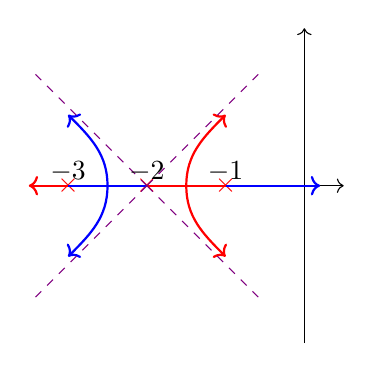
\begin{tikzpicture}[scale=1]
		\coordinate (o) at (0,0);
		\coordinate (ox) at (0.5,0);
		\draw[->] (-3,0) -- (ox);
		\draw[->] (0,-2) -- (0,2);
		%\draw (o) node[below left] {$o$};
		\draw[thick,red] (-1,0) node {$\times$};
		\draw[thick,red] (-2,0) node {$\times$};
		\draw[thick,red] (-3,0) node {$\times$};
		
		\draw [blue,thick] (-3,0)--(-2,0);
		\draw [red,thick] (-2,0)--(-1,0);
		\draw [->,red,thick] (-3,0)--(-3.5,0);
		\draw [->,blue,thick] (-1,0)--(0.2,0);
		
		\draw [->,red,thick](-1.5,0) to [out=90,in=-135](-1,0.9);
		\draw [->,red,thick](-1.5,0) to [out=-90,in=135](-1,-0.9);
		\draw [->,blue,thick](-2.5,0) to [out=90,in=-45](-3,0.9);
		\draw [->,blue,thick](-2.5,0) to [out=-90,in=45](-3,-0.9);
		
		
		\draw [violet,dashed] (-2,0)--+(45:2);
		\draw [violet,dashed] (-2,0)--+(-45:2);
		\draw [violet,dashed] (-2,0)--+(135:2);
		\draw [violet,dashed] (-2,0)--+(-135:2);
		
		%\draw (-1,0) node[below=1em] {$-1$};
		\draw (-1,0) node[xshift=0em ,yshift=0.5em] {$-1$};
		\draw (-2,0) node[xshift=0em ,yshift=0.5em] {$-2$};
		\draw (-3,0) node[xshift=0em ,yshift=0.5em] {$-3$};
		\end{tikzpicture}
		
		计算分离点,由
		$$
		\frac{d}{ds}(k+(s+1)(s+2)(s+3))=0
		$$
		得
		$$
		\lambda=-2\pm\frac{1}{\sqrt{3}}
		$$
		分别将其代入特征方程,可得:
		$$
		\begin{cases}
		k=\frac{2}{3\sqrt{3}} & (\lambda=-2+\frac{1}{\sqrt{3}})\\
		k=-\frac{2}{3\sqrt{3}} & (\lambda=-2-\frac{1}{\sqrt{3}})
		\end{cases}
		$$
		因此,当$-\frac{2}{3\sqrt{3}}\leqslant k \leqslant \frac{2}{3\sqrt{3}}$ 时,闭环系统根位于实轴负半轴,即系统超调量为0。
	}
}


%-------------------------------------------------------
\clearpage

\end{document}
